\scanpage{45}
\deleted{théorème de finitude}

théorème d'acyclicité locale\quad local acyclicity theorem\quad XV 2.1, XIX 4.1

couple régulier de schémas\quad regular pair of schemes\quad XIX 3.1

théorème de changement de base par morphisme régulier\quad base change theorem for regular base change morphism\deleted{e}\quad XIX 4.2

$\unsure{\deleted{d}\handwritten{\delta}|\deleted{Q}\handwritten{\delta}|\handwritten{\delta}}(F,f,y)$\qquad XIX 6.0
\figure{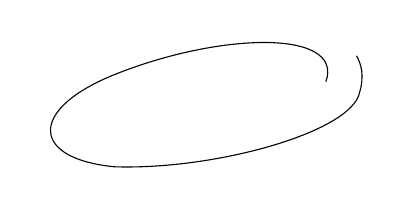
\begin{tikzpicture}
\draw (1.58,.4) .. controls (1.82,1.08) and (.18,1.03) .. (-1.18,.46) .. controls (-2.2,.02) and (-2.15,-.58) .. (-1.1,-.68) .. controls (.2,-.72) and (1.92,-.23) .. (2.01,.27) .. controls (2.07,.48) and (2.03,.62) .. (1.97,.73);
\end{tikzpicture}}

formellement séparable (k-algèbre - )\quad formally separable \inserted{\handwritten{k-}}algebra\quad XIX 6.7.\inserted{\handwritten{0}}
\figure{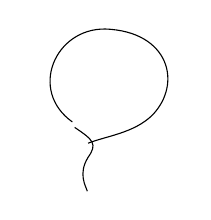
\begin{tikzpicture}
\draw (-.47,-.25) .. controls (-1.03,.15) and (-.69,.94) .. (-.05,.93) .. controls (.76,.9) and (.93,.24) .. (.55,-.16) .. controls (.32,-.39) and (-.04,-.43) .. (-.27,-.52);
\draw (-.44,-.32) .. controls (-.2,-.48) and (-.15,-.53) .. (-.27,-.7) .. controls (-.4,-.91) and (-.3,-1.06) .. (-.28,-1.13);
\end{tikzpicture}}
\figure{\begin{tikzpicture}
\draw[line cap=round] (-.48,.42) .. controls (-.7,.2) and (-.68,-.04) .. (-.38,-.08) .. controls (-.13,-.12) and (.12,-.01) .. (.34,-.1) .. controls (.56,-.19) and (.45,-.49) .. (.43,-.8);
\end{tikzpicture}}

\begin{tabular}{@{}lll@{}}
\handwritten{étendue algébrique}&\handwritten{$\overline{\underline{\mathrm{VIII}}}$ 10.2\unsure{.|,}}&\handwritten{algebraic spread}\\
\handwritten{espace algébrique}&\handwritten{$\overline{\underline{\mathrm{VIII}}}$ 10.4.}&\handwritten{algebraic space}
\end{tabular}
\figure{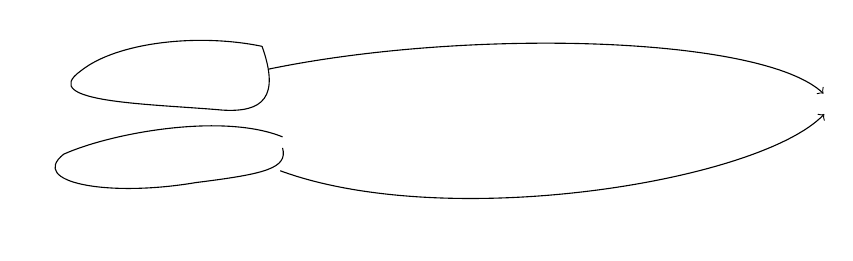
\begin{tikzpicture}
\draw (1.2,.43) .. controls (.38,.6) and (-.65,.48) .. (-1.1,.12) .. controls (-1.68,-.29) and (-.19,-.3) .. (.7,-.38) .. controls (1.21,-.41) and (1.43,-.22) .. (1.2,.43);
\draw (1.46,-.72) .. controls (.7,-.41) and (-.72,-.67) .. (-1.32,-.94) .. controls (-1.77,-1.3) and (-.76,-1.49) .. (.36,-1.3) .. controls (1.24,-1.19) and (1.53,-1.12) .. (1.46,-.86);
\draw[->] (1.28,.14) .. controls (3.79,.66) and (7.54,.57) .. (8.33,-.17);
\draw[->] (1.43,-1.15) .. controls (3.55,-1.93) and (7.51,-1.29) .. (8.34,-.43);
\end{tikzpicture}}
% archive sheet number: 44
